\chapter{Introduzione}

Expiration Date è un'applicazione nata per permettere la gestione completa di tutto ciò che riguarda i prodotti alimentari; con essa è infatti possibile gestire gli aspetti relativi:
\begin{itemize}
  \item alla lista della spesa (prodotti che si desidera acquistare)
  \item alla dispensa (prodotti già posseduti)
  \item alle ricette
\end{itemize}

\begin{figure}[H]
  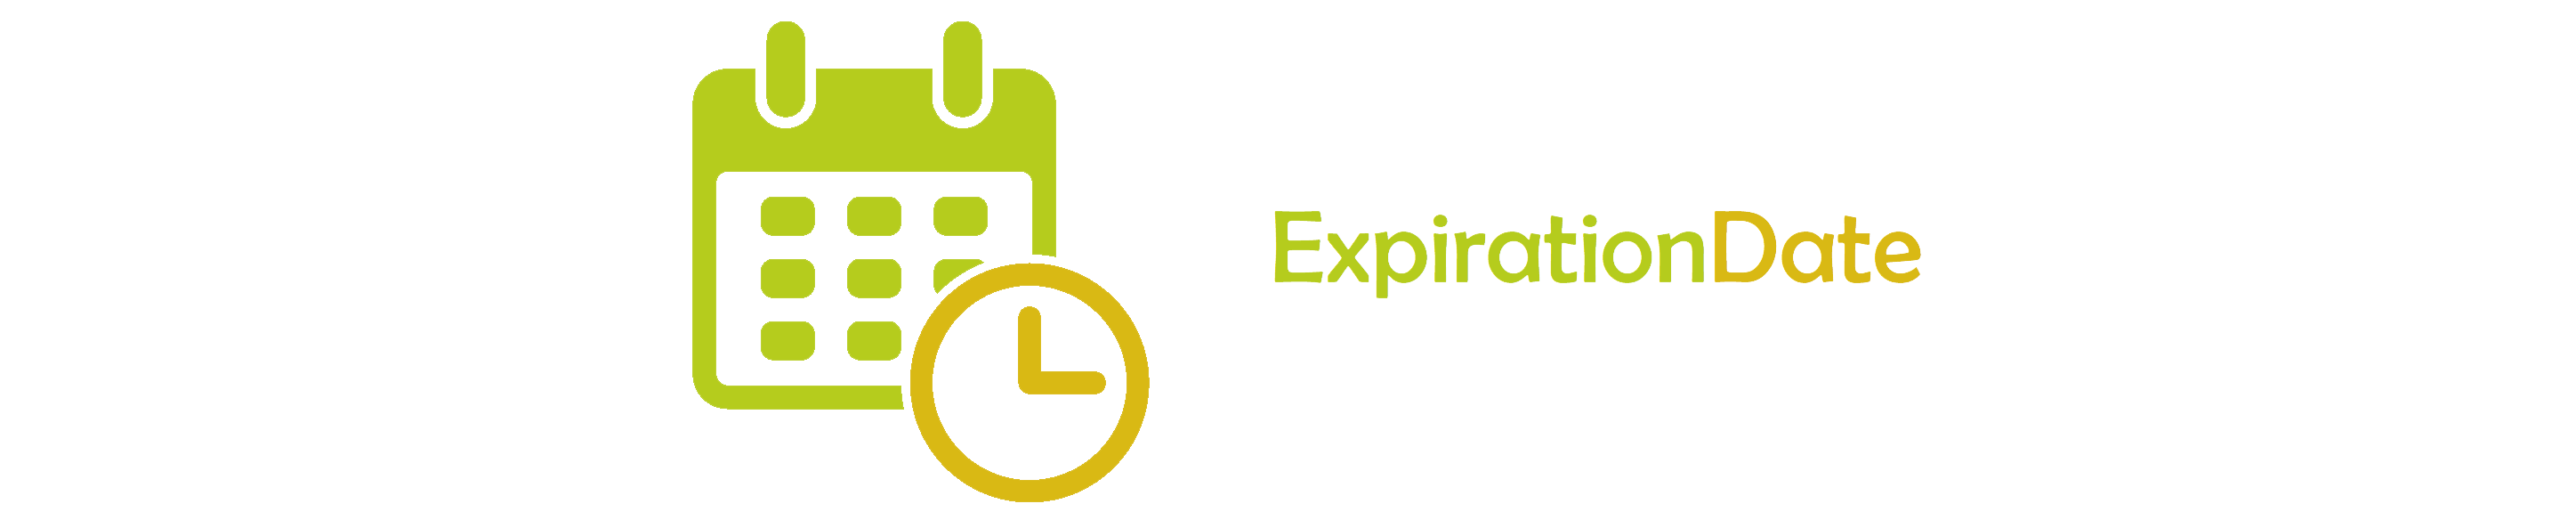
\includegraphics[width=\linewidth]{images/app-logo.png}
  \caption{Logo dell'applicazione.}
  \label{fig:applogo}
\end{figure}

Nel seguito verranno illustrati:
\begin{itemize}
\item i requisiti (funzionali e non funzionali) alla base dello sviluppo dell'applicazione
\item una panoramica generale dell'applicazione, con particolare attenzione all'interfaccia grafica
\item i diagrammi UML (Unified Modeling Language) che descrivono nel dettaglio le funzionalità dell'applicazione e la sua business logic
\item i design patterns implementati, le motivazioni e i vantaggi del loro impiego
\item la tecnica ORM (Object-Relational Mapping) per la gestione della persistenza dei dati e l'interfacciamento con il database
\end{itemize}